%!TEX program=xelatex
\documentclass{beamer}
\usetheme{focus}
% Full instructions available at:
% https://github.com/elauksap/focus-beamertheme

\usepackage{ctex}
\usepackage{multirow}

\usepackage{listings}
\usepackage{golang}
\usepackage{xcolor}

\title{Go并发元件}
%\subtitle{Subtitle}
\author{黎相敏}
\titlegraphic{
\includegraphics[scale=1.25]{focuslogo.pdf}}
\institute{上海观源信息科技有限公司 \\ 上海市闵行区紫竹科技园4号楼303B}
\date{12/01/2019}

\lstset{ % add your own preferences
    frame=trBL, %single,
    basicstyle=\ttfamily\scriptsize,
    keywordstyle=\color{red},
    numbers=left,
    numbersep=8pt,
    showstringspaces=false, 
    stringstyle=\color{blue},
    tabsize=2,
    language=golang % this is it !
}
\renewcommand{\lstlistingname}{代码片段}% Listing -> 代码片段

% command macros to save typing
\newcommand{\channel}{\texttt{channel}}
\newcommand{\code}[1]{\textcolor{magenta}{\texttt{#1}}}
\newcommand{\Cond}{\texttt{Cond}}
\newcommand{\Mutex}{\texttt{Mutex}}
\newcommand{\Once}{\texttt{Once}}
\newcommand{\Pool}{\texttt{Pool}}
\newcommand{\RWMutex}{\texttt{RWMutex}}
\newcommand{\select}{\texttt{select}}
\newcommand{\WaitGroup}{\texttt{WaitGroup}}

\begin{document}
    \begin{frame}
        \maketitle
    \end{frame}

    \begin{frame}{大纲}
        \tableofcontents
    \end{frame}

    \section{基本术语}
\begin{frame}{分叉--汇合(Fork-Join)模型}
  \begin{columns}
      \column{.5\textwidth}
        \begin{itemize}
          \item 程序执行过程中,\alert{父线程}可以分叉出与其并发执行的\alert{子线程}
          \item \alert{汇合点}: 子线程从独立执行到汇合回父线程的时间点
        \end{itemize}

      \column{.5\textwidth}
      \begin{figure}
        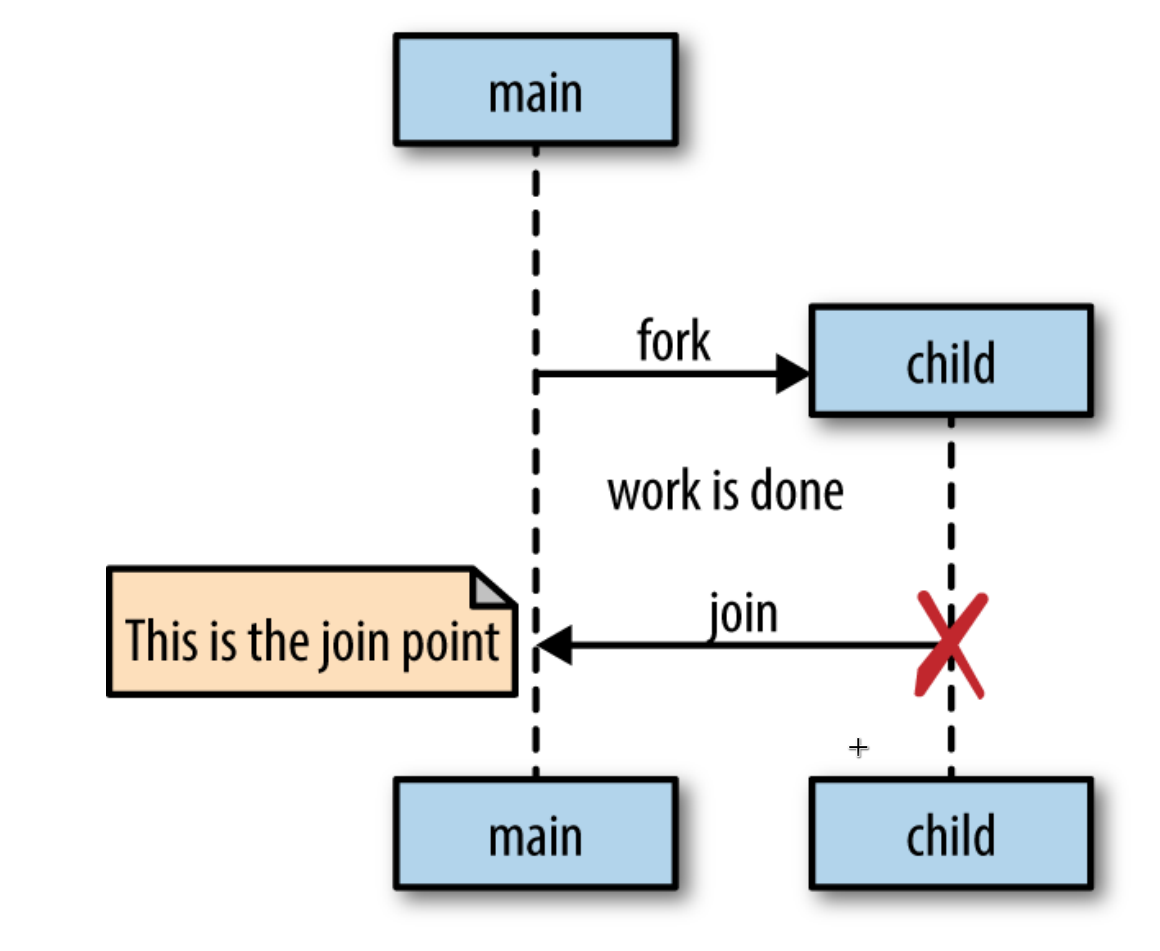
\includegraphics[width=\textwidth]{images/fork-join.png}
        \caption{分叉--汇合模型}
      \end{figure}
  \end{columns}
\end{frame}

\begin{frame}[fragile]{错误设置的汇合点}
\begin{lstlisting}[caption={不正确的汇合点引发竞态},label={wrong-join}]
sayHello := func() {
  fmt.Println("hello")
}
go sayHello()
// continue doing other things
\end{lstlisting}

    \alert{以上程序的输出结果是不确定的}。因为协程由 Go 运行时创建和调度,\code{sayHello}协程没能通过合适的汇合点和主协程进行汇合。因此,如果被调度之前主协程已退出,\code{sayHello}就无法获得执行的机会

    \begin{exampleblock}{温馨提示}
        \textbf{正确设置的汇点}能确保程序正确性并消除潜在的\alert{竞态} 
    \end{exampleblock}
\end{frame}

\begin{frame}[fragile]{纠正的汇合点}
为上述程序设置正确的汇合点,\texttt{sayHello}必须和主协程\textbf{同步},使自己能在主协程退出之前与其汇合,解决方案之一如\lstlistingname~\ref{lst-ok-join}

\begin{lstlisting}[caption={利用同步确保\texttt{sayHello}在主协程退出之前与其汇合},label=lst-ok-join]
var wg sync. WaitGroup
sayHello := func() {
  defer wg.Done()
  fmt.Println("hello")
}
wg.Add(1)
go sayHello()
wg.Wait()  // 汇合点

// 输出:
// hello    
\end{lstlisting}

\alert{可见,分叉---汇合模型下并发编程的正确性依赖于数据同步}
\end{frame}

\begin{frame}{数据同步方式}
\texttt{go}语言实现数据同步操作提供了两种方式
\begin{itemize}
    \item 传统地,\alert{共享内存型同步模式},常用元件分布在\texttt{sync}包
    \item \alert{基于顺序进程通信(CSP)}的消息传递实现数据同步,主要元件为通道\texttt{channel}及\texttt{select}语句
\end{itemize}
\end{frame}

    \section{sync包}
  \begin{frame}{基本元件}
  \texttt{sync}包维护着用于同步底层内存访问的元件,包括
  \begin{itemize}
      \item \WaitGroup
      \item 通用锁\Mutex 和读写锁\RWMutex
      \item 条件信号量\Cond
      \item \Once
      \item 池\Pool
  \end{itemize} 
  \end{frame}
    \subsection{\WaitGroup}
\begin{frame}[fragile]{\WaitGroup}
   \textbf{用途}: 等待一批并发操作结束,\alert{操作的结果不是关心的重点或者能够通过其他途径收集} 

   \begin{columns}[t]
       \column{0.6\textwidth}
\begin{lstlisting}[xleftmargin=8pt]
var wg sync.WaitGroup

wg.Add(1)
go func() {
  defer wg.Done()
  fmt.Println("Alice sleeping...")
  time.Sleep(1)
}()

wg.Add(1)
go func() {
  defer wg.Done()
  fmt.Println("Bob sleeping...")
  time.Sleep(2)
}()
wg.Wait()
fmt.Println("Both are awaken.")
\end{lstlisting}

       \column{0.4\textwidth}
\begin{lstlisting}[firstnumber=last,xleftmargin=16pt]
// 输出:
// Bob sleeping...
// Alice sleeping...
// Both are awaken.
\end{lstlisting}
   \end{columns}
\end{frame}

\begin{frame}{\WaitGroup}
    \WaitGroup 可看作一个\alert{协程安全}的计数器

    \begin{itemize}
        \item 通过 \code{Add(x)}加上特定数\code{x}
        \item 通过 \code{Done()}使其减1
        \item \code{Wait()}使其一直阻塞直至计数器置零
    \end{itemize}

    \pause
    \begin{alertblock}{温馨提示}
        \code{Add()}需要在\WaitGroup 协调的协程之外(一般是主协程)调用,否则将引入\alert{竞态}
    \end{alertblock}
\end{frame}
    \subsection{\Mutex 和\RWMutex }
\begin{frame}{基本介绍}
    \begin{itemize}
        \item \Mutex 是``Mutual Exclusion''的缩写
        \item \textbf{用途}: 保护程序的\alert{关键区域}---需要排他地存取共享资源的程序片段
        \item \Mutex 和\RWMutex 要求开发者必须以\alert{特定的方式}访问内存以保证数据的同步
    \end{itemize}
\end{frame}

\begin{frame}[fragile]{示例}
\begin{lstlisting}[caption={\Mutex 使用示例}]
var count int
var lock sync.Mutex

increment := func() {
  lock.Lock()
  defer lock.Unlock()
  count++
  fmt.Printf("Incrementing: %d\n", count)
}
decrement := func() {
  lock.Lock() // 请求对关键区域--count变量的存取
  defer lock.Unlock()  // 放弃对关键区域的排他存取权利
  count--
  fmt.Printf("Decrementing: %d\n", count)
}
\end{lstlisting}
\end{frame}

\begin{frame}[fragile]{示例(续)}
    \begin{columns}[t]
        \begin{column}{0.5\textwidth}
\begin{lstlisting}[caption={\Mutex 使用示例(续)},firstnumber=last,xleftmargin=8pt]
// Increment
var arithmetic sync.WaitGroup
for i := 0; i <= 2; i++ {
  arithmetic.Add(1)
  go func() {
    defer arithmetic.Done()
    increment()
  }()
}
// Decrement
for i := 0; i <= 2; i++ {
  arithmetic.Add(1)
  go func() {
    defer arithmetic.Done()
\end{lstlisting}
        \end{column}
        \begin{column}{0.5\textwidth}
\begin{lstlisting}[caption={\Mutex 使用示例(续)},firstnumber=last,xleftmargin=8pt]
    decrement()
  }()
}
arithmetic.Wait()
fmt.Println("Arithmetic complete.")

// 输出:
// Decrementing: -1
// Incrementing: 0
// Incrementing: 1
// Decrementing: 0
// Decrementing: -1
// Incrementing: 0
// Arithmetic complete.
\end{lstlisting}
        \end{column}
    \end{columns}
\end{frame}

\begin{frame}{温馨提示}
    \begin{itemize}
        \item 锁\texttt{m}的\texttt{Lock()}调用之后应有配对的\texttt{defer m.UnLock()}语句
        \item \alert{进出关键区域的代价是昂贵的}
    \end{itemize}    
\end{frame}

\begin{frame}{读写锁\RWMutex }
    \alert{在写锁未被锁定之前},读写锁能够满足任意共存的读锁请求

    示例代码参见\href{https://github.com/sammyne/concurrency-in-go/blob/master/chapter03/sync.pkg/mutex/rwlock.go}{\Mutex 和\RWMutex 性能对比},具体结果如下图所示,\alert{可见,性能替身没有想象中的那么明显}

    \begin{figure}
        \centering
        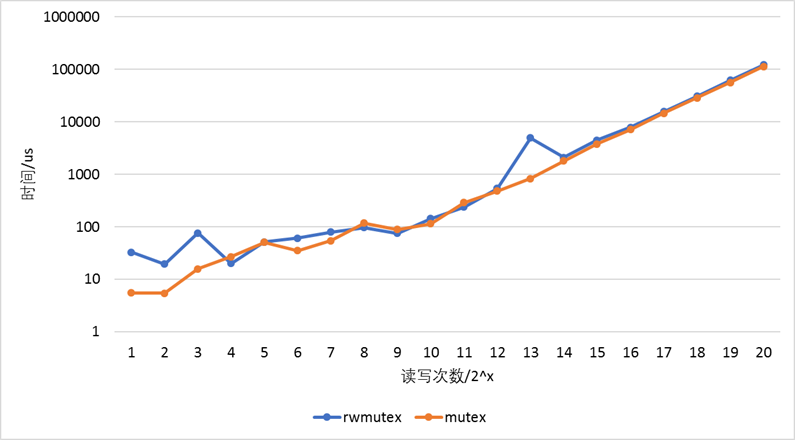
\includegraphics[width=0.7\textwidth]{images/rwmutex-vs-mutex.png}
        \caption{\Mutex 和\RWMutex 性能对比结果}
    \end{figure}
\end{frame}

\iffalse
\begin{frame}{读写锁\RWMutex }
    \alert{在写锁未被锁定之前},读写锁能够满足任意共存的读锁请求

    示例代码参见\href{https://github.com/sammyne/concurrency-in-go/blob/master/chapter03/sync.pkg/mutex/rwlock.go}{\Mutex 和\RWMutex 性能对比}

    程序的输出结果类似
    \begin{columns}
        \column{0.5\textwidth}
            \begin{table}
                \centering
                \caption{\Mutex 和\RWMutex 性能对比}
                \begin{tabular}{lll}
                    \hline
                    Readers  &RWMutex       &Mutex  \\
                    \hline
                    1        &32.87µs       &5.541µs \\
                    2        &19.603µs      &5.439µs \\
                    4        &76.62µs       &15.886µs \\
                    8        &20.201µs      &26.892µs \\
                    16       &51.558µs      &50.657µs \\
                    32       &61.313µs      &34.999µs \\
                    \hline
                \end{tabular}
            \end{table}

        \column{0.5\textwidth}
            \begin{table}
                \centering
                \caption{\Mutex 和\RWMutex 性能对比(续)}
                \begin{tabular}{lll}
                    \hline
                    Readers  &RWMutex       &Mutex  \\
                    \hline
                    64       &79.628µs      &54.763µs \\
                    128      &96.749µs      &118.701µs \\
                    256      &75.414µs      &89.375µs \\
                    512      &142.882µs     &114.705µs \\
                    1024     &239.471µs     &289.861µs \\
                    2048     &540.809µs     &479.173µs \\ 
                    \hline
                \end{tabular}
            \end{table}
    \end{columns}
\end{frame}

\begin{frame}{读写锁\RWMutex }
            \begin{table}[htbp!]
                \caption{\Mutex 和\RWMutex 性能对比(续)}
                \begin{tabular}{lll}
                    \hline
                    Readers  &RWMutex       &Mutex  \\
                    \hline
                    2048     &540.809µs     &479.173µs \\ 
                    4096     &4.982512ms    &827.095µs \\
                    8192     &2.09599ms     &1.790277ms \\
                    16384    &4.47045ms     &3.820926ms \\
                    32768    &7.911863ms    &7.163938ms \\
                    65536    &15.689641ms   &14.66057ms \\
                    131072   &31.016011ms   &28.674835ms \\
                    262144   &62.493129ms   &56.609731ms \\
                    524288   &121.927969ms  &113.786247ms \\   
                    \hline
                \end{tabular}
            \end{table} 
\end{frame}
\fi
    \subsection{条件信号量\Cond}
\begin{frame}{条件信号量\Cond}
    \begin{itemize}
        \item \textbf{用途}: 协程用于等待或通知特定事件发生的消息中心
        \item 这里的事件只在两个或更多协程之间传递事件发生的事实本身,\alert{无法承载其他信息}
    \end{itemize}
\end{frame}

\begin{frame}[fragile]{使用场景}
   没有借助条件信号量实现事件通知的两种方式
   
   \begin{enumerate}
       \item \code{for}循环等到为止: 无限占用 CPU 内核,\alert{无法被调度}
\begin{lstlisting}
for conditionTrue() == false { }    
\end{lstlisting}
       \item 利用主动睡眠提供可被抢占机会: \alert{效率不高,且难以准确设置睡眠的时长}:太长降低性能,太短消耗太多 CPU 时间    
\begin{lstlisting}
for conditionTrue() == false {
  time. Sleep(1*time.Millisecond)
}
\end{lstlisting}
   \end{enumerate}
\end{frame}

\begin{frame}[fragile]{使用场景}
   借助\Cond 实现事件通知的更优
\begin{lstlisting}
c := sync.NewCond(&sync.Mutex{})

c.L.Lock()
for conditionTrue() == false {
  c.Wait()
}
c.L.Unlock()
\end{lstlisting}

\begin{itemize}
    \item \code{Wait()}促使协程进入阻塞状态,挂起当前协程,为其他协程腾出在系统级线程执行的机会
    \item \code{Wait()}内部执行过程会先调用所绑定锁的\code{Unlock()},而在收到需要的信号后、退出执行前再次执行\code{Lock()}重新获得对锁的控制权
\end{itemize}

另一个例子是\mhref{https://github.com/sammyne/concurrency-in-go/blob/master/chapter03/sync.pkg/cond/queue.go}{玩具级的限定容量队列}
\end{frame}

\begin{frame}{两种通知方式: \code{Signal}和\code{Broadcast}}
   \begin{itemize}
       \item Go 运行时维护着等待信号的协程队列(先进先出)
       \item \code{Signal()}调用后,Go 运行时只会通知等待最久的那个协程并将其出列
       \item \code{Broadcast()}的调用则会(逐一?并发?)通知所有等待的协程
       \item \Cond 的性能要比\channel 的高
   \end{itemize} 

   某些需求场景下,基于\Cond 的实现会比基于通道\channel 简洁很多。例如,\href{https://github.com/sammyne/concurrency-in-go/blob/master/chapter03/sync.pkg/cond/boardcast.go}{按钮点击事件的通知}
\end{frame}
    \subsection{\Once }
\begin{frame}[fragile]{\Once }
  \text{用途}: 确保某个操作最多只被执行一次

\begin{columns}[T]
    \column{.45\textwidth}    
\begin{lstlisting}[caption={\Once 使用样例},xleftmargin=8pt]
var count int
increment := func() {
  count++
}

var once sync.Once

var increments sync.WaitGroup
increments.Add(100)
for i := 0; i < 100; i++ {
  go func() {
    defer increments.Done()
    once.Do(increment)
  }()
\end{lstlisting}

    \column{.5\textwidth}    
\begin{lstlisting}[caption={\Once 使用样例},firstnumber=last,xleftmargin=8pt]
}

increments.Wait()
fmt.Printf("Count is %d\n", count)

// 输出:
// Count is 1    
\end{lstlisting}
\end{columns}
\end{frame}

\begin{frame}[fragile]{注意事项}
  \begin{itemize}
      \item \Once 确保的目标操作是通过自己的\texttt{Do()}函数注册的第一个回调函数
      \item \Once 内部使用锁,在回调函数调用前请求锁,而在调用返回前释放锁,需要留意不同回调函数之间的依赖性,避免死锁
  \end{itemize}  

\begin{lstlisting}[caption={\Once 的使用不当导致死锁}]
var onceA, onceB sync. Once
var initB func()
initA := func() { onceB. Do(initB) }
initB = func() { onceA. Do(initA) }

onceA. Do(initA)    

// 输出:
// fatal error: all goroutines are asleep - deadlock!
\end{lstlisting}
\end{frame}
    \subsection{池\Pool }
\begin{frame}{池\Pool }
    \begin{itemize}
        \item \text{用途}: 池模式创建并导出特定数目或一批资源以被第三方使用
        \item 3个基本方法
            \begin{description}
                \item[New] 创建资源实例
                \item[Get] 调用时,如果池有可用的实例,则将其直接返回给请求方,否则调用New方法实时创建一个然后将其返回给请求方
                \item[Put] 将服务完毕的实例放回池缓存以被其他进程使用
            \end{description}
    \end{itemize}
\end{frame}

\begin{frame}[fragile]{实例}
    利用池创建对象,\alert{使用完毕后重新放回池中},从而节省对象的创建
\begin{lstlisting}
myPool := &sync.Pool{
  New: func() interface{} {
    fmt.Println("Creating new instance.")
    return struct{}{}
  },
}
myPool.Get()
instance := myPool.Get()
myPool.Put(instance)
myPool.Get()

// 输出:
// Creating new instance.
// Creating new instance.
\end{lstlisting}

另一个例子是\href{https://github.com/sammyne/concurrency-in-go/blob/master/chapter03/sync.pkg/pool/basic2.go}{使用池缓存资源以节省内存空间}

\end{frame}

\begin{frame}{更多使用场景}
    预存一批能够快速响应(初始化比较漫长)的服务提供方,相关代码参见
    \begin{itemize}
        \item \href{https://github.com/sammyne/concurrency-in-go/blob/master/chapter03/sync.pkg/pool/slow_network_service_benchmark_test.go}{没有使用池预存对象的方式}
        \item \href{https://github.com/sammyne/concurrency-in-go/blob/master/chapter03/sync.pkg/pool/slow_network_service_benchmark_test.go}{使用池预存对象的方式}
    \end{itemize}

    对比结果是:使用缓存池的方式快了近 1000 倍
\end{frame}

\begin{frame}{注意事项}
\begin{exampleblock}{适用条件}
    \begin{itemize}
        \item 为并发的进程提供服务对象,这些对象需要满足
            \begin{itemize}
                \item 在初始化后很快就被抛弃
                \item 或创建会对内存影响不小
            \end{itemize}
    \end{itemize}
\end{exampleblock}    

\begin{alertblock}{不适用条件}
   所需服务对象不是同态的---部分时间会被浪费在对象的类型转换上 
\end{alertblock}
\end{frame}

\begin{frame}{\Pool 小结}
    \begin{itemize}
        \item 初始化\Pool 时,创建一个\texttt{New}成员
        \item 不要对\texttt{Get()}返回的对象状态做任何前提假设
        \item 不要忘记利用\texttt{Put()}将服务对象再次缓存以重用
        \item 池中对象应基本同态,即类型相同    
    \end{itemize}
\end{frame}
    
    \section{通道\channel }
\begin{frame}{用途和种类}
    \begin{itemize}
        \item \textbf{用途}: 以线程安全的方式实现不同协程之间的通信 
        \item 通道在声明时指定其数据流向
            \begin{itemize}
                \item \alert{读写}\quad 默认,例如,\code{xStream := make(chan int)}
                \item \alert{只读}\quad 将<-箭头放在\code{chan}关键字的左边,例如,\code{yStream := make(<-chan int)}
                \item \alert{只写}\quad 将<-箭头放在\code{chan}关键字的右边,例如,\code{zStream := make(chan<- int)}
            \end{itemize}
    \end{itemize}

    \begin{exampleblock}{温馨提示}
        go 会在必要时隐式地将单向通道(只读/只写)转为双向通道(读写) 
    \end{exampleblock}
\end{frame}

\begin{frame}[fragile]{数据类型与传递}
    \begin{itemize}
        \item 通道传递的数据类型可以被指定
        \item 对于一个可读通道\code{c},可以利用表达式\code{c <- x}将值\code{x}放到通道里
        \item 对于一个可写通道\code{c},可以利用表达式\code{y <- c}从通道里取出值\code{y}
    \end{itemize}
\begin{lstlisting}[caption={通道数据传递样例}]
stringStream := make(chan string)
go func() {
  stringStream <- "Hello channels!"
}()
fmt.Println(<-stringStream)

// 输出:
// Hello channels!    
\end{lstlisting}    
\end{frame}

\begin{frame}[fragile]{导致编译错误的操作}
\begin{itemize}
    \item 对只读通道的写操作
\begin{lstlisting}
readStream := make(<- chan interface{})
readStream <- struct{}{}

// 输出:
// invalid operation: readStream <- struct {} literal 
// (send // to receive-only type <-chan interface {})    
\end{lstlisting}
        \item 对只写通道的读操作
\begin{lstlisting}
writeStream := make(chan<- interface{})
<- writeStream

// 输出:
// invalid operation: <-writeStream (receive from 
// send-only type chan<- interface {})
\end{lstlisting}
\end{itemize}
\end{frame}

\begin{frame}{阻塞性}
    \begin{itemize}
        \item 任何尝试向容量已满的通道发送数据的协程会等待直至通道有剩余空间
        \item 任何尝试向空通道读数据的协程都会等待直至有一个值进入通道
    \end{itemize}
\end{frame}

\begin{frame}[fragile]{读操作的两种方式}
    \begin{itemize}
        \item 只返回一个值: 从通道传输下来的数值
        \item 返回一个值\code{x}和一个布尔值\code{closed}
            \begin{itemize}
                \item \code{x}表示从通道传输下来的数据
                \item \code{closed=false}表示\code{x}是由于通道已关闭其容量为空而返回的所声明类型的默认值
                \item \code{closed=false}则表示\code{x}是从别处写入通道的值
            \end{itemize}
    \end{itemize}

\begin{lstlisting}[caption={通道的两种读取操作}]
stringStream := make(chan string)
go func() {
  stringStream <- "Hello channels!"
}()

salutation, ok := <-stringStream
fmt.Printf("(%v): %v", ok, salutation)

// 输出:
// (true): Hello channels!
\end{lstlisting}
\end{frame}

\begin{frame}{通道的关闭}
    \begin{itemize}
        \item \code{close(c)}函数调用可关闭通道\code{c}
        \item 可读通道能够满足无限的读请求(即使通道已被关闭)
    \end{itemize}
\end{frame}

\begin{frame}[fragile]{设计模式1: \code{for...range}遍历}
    \code{range}和\code{for}关键字组合可以通道作为实参,并在通道关闭时自动跳出循环
\begin{lstlisting}
intStream := make(chan int)

go func() {
    defer close(intStream)
    for i := 1; i <= 5; i++ {
    intStream <- i
    }
}()

for integer := range intStream {
    fmt.Printf("%v ", integer)
}

// 输出:
// 1 2 3 4 5 
\end{lstlisting}    
\end{frame}

\begin{frame}[fragile]{设计模式2: 作为取消信号}
    以通道的关闭为信号通知多个协程
\begin{lstlisting}
begin := make(chan interface{})
var wg sync.WaitGroup
for i := 0; i < 3; i++ {
    wg.Add(1)
    go func(i int) {
        defer wg.Done()
        <-begin
        fmt.Printf("%v has begun\n", i)
    }(i)
}
fmt.Println("Unblocking goroutines...")
close(begin)
wg.Wait()

// Unblocking goroutines...
// 1 has begun
// 0 has begun
// 2 has begun
\end{lstlisting}
\end{frame}

\begin{frame}{容量}
    \begin{itemize}
        \item 通道根据容量可划分为 2 种类型:\alert{非缓存型}和\alert{缓存型}
        \item 非缓存型: 声明时不指定容量或指定容量为 0
        \item 缓存型: 通道在初始化时被赋予大于 0 的容量
            \begin{itemize}
                \item 给定容量为\code{n},对通道\code{c}可同时支持\code{n}个写操作
                \item 可作为一个内存型消息队列实现并发进程间的通信
                \item 通道为空且有挂起的等待协程时,新值的传入会绕过通道直接传给等待协程
                \item 这类通道容易\alert{导致过早优化问题}和\alert{隐藏死锁问题}
            \end{itemize}
    \end{itemize}
    通道的满和空都是相对与通道的容量而言的 


    在预知通道需要支持的并发写操作次数\code{n}时,容量大小为\code{n}的缓存型通道可以使得写操作尽可能快地执行,例如,\href{https://github.com/sammyne/concurrency-in-go/blob/master/chapter03/channels/buffered_channel.go}{缓存型通道作为消息队列}
\end{frame}

\begin{frame}[fragile]{\texttt{nil}通道}
    给定\code{nil}通道\code{c}
    \begin{itemize}
        \item 对\code{c}的读操作会阻塞进程(尽管并不一定会导致死锁??)
\begin{lstlisting}
    fatal error: all goroutines are asleep - deadlock!
\end{lstlisting}
        \item 对\code{c}的写操作也会阻塞进程
\begin{lstlisting}
fatal error: all goroutines are asleep - deadlock!
\end{lstlisting}
        \item 关闭\code{c}会触发\code{panic}
\begin{lstlisting}
    panic: close of nil channel 
\end{lstlisting}
    \end{itemize}
\end{frame}

\begin{frame}{对通道不同操作的后果}

\begin{figure}
    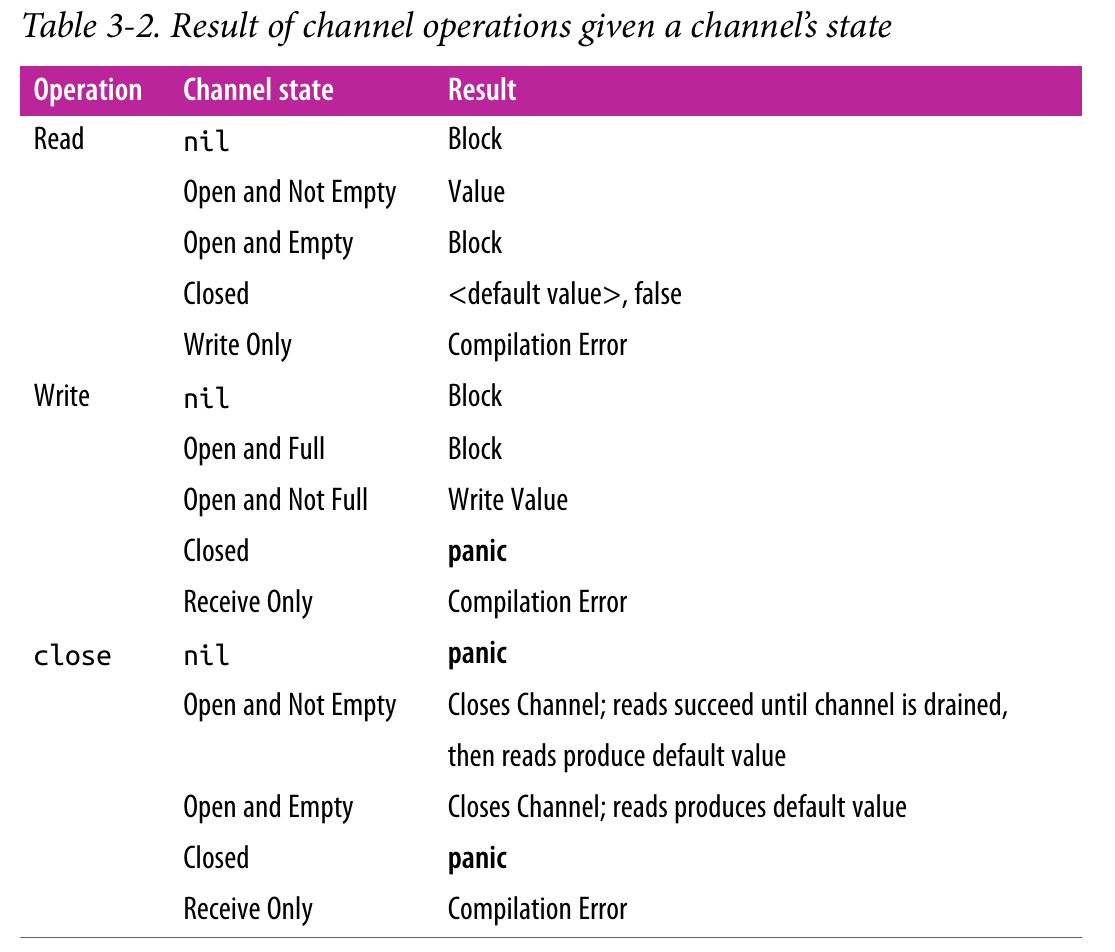
\includegraphics[width=0.5\textwidth]{images/channel-operations.png}
    \caption{对通道不同操作的后果}
\end{figure}

    由表可知,
\begin{itemize}
    \item 阻塞协程的操作有 3 种
    \item 导致协程恐慌的操作有 3 种
\end{itemize}
\end{frame}

\begin{frame}{上下文}
    通道的正确使用需要有合理的上下文环境,而为通道赋予正确的所有权协助创造这种环境

    \alert{通道的所有权应该属于负责初始化、写入数据和关闭通道的协程}
    
    通过这种规则限定
    \begin{itemize}
        \item \alert{所有者}持有对通道的\alert{读写权限},并负责
            \begin{itemize}
                \item 初始化通道
                \item 执行写操作或将通道所有权转移给其他协程
                \item \alert{关闭通道}
                \item 将以上 3 项封装为一个只读通道暴露给消费者
            \end{itemize}
        \item \alert{消费者}则对通道只有\alert{读权限},只需关心
            \begin{itemize}
                \item 监听通道的关闭
                \item 负责处理任何情况下的阻塞
            \end{itemize}
    \end{itemize} 
\end{frame}

\begin{frame}[fragile]{基于通道实现的所有者---消费者样例}
    \begin{columns}[t]
        \column{0.65\textwidth}
\begin{lstlisting}[xleftmargin=8pt]
chanOwner := func() <-chan int {
    resultStream := make(chan int, 5)
    go func() {
        defer close(resultStream)
        for i := 0; i <= 5; i++ {
        resultStream <- i
        }
    }()
    return resultStream
}
    
resultStream := chanOwner()
for result := range resultStream {
    fmt.Println("Received:", result)
}
fmt.Println("Done!")

\end{lstlisting}
        \column{0.3\textwidth}
\begin{lstlisting}[firstnumber=last,xleftmargin=8pt]
// 输出:
// Received: 0
// Received: 1
// Received: 2
// Received: 3
// Received: 4
// Received: 5
// Done!    
\end{lstlisting}
    \end{columns}
\end{frame}
    \section{\select 语句}
\begin{frame}[fragile]{\select 语句}
    \begin{itemize}
        \item \select 语句负责绑定通道到
            \begin{itemize}
                \item 局部的类型或单个函数
                \item 全局范围内多个系统组件
            \end{itemize}
        \item 借助\select 语句安全地利用通道实现诸如\alert{取消}、\alert{超时}(\lstlistingname~\ref{lst-select-based-timeout})、\alert{等待}和\alert{默认值}等概念
        \item 空\select 语句(\code{select \{\}})等价于一个死循环,会永远阻塞
    \end{itemize}

\begin{lstlisting}[caption={基于\select 实现超时退出},label=lst-select-based-timeout]
var c <-chan int
select {
case <-c:
case <-time.After(1 * time.Second):
    fmt.Println("Timed out.")
}

// 输出:
// Timed out.
\end{lstlisting}
    
\end{frame}

\begin{frame}{\texttt{case}子句的选择公平性}
    \begin{itemize}
        \item 不同于\code{switch}语句,对于\select 语句
            \begin{itemize}
                \item \code{case}子句不会线性地从上往下执行
                \item 在没有任何满足条件的\code{case}子块时会一直阻塞
                \item Go 运行时会随机均匀地选择非阻塞的\code{case}子句执行
            \end{itemize}
    \end{itemize}

\code{case}语句指明的所有通道读写操作会被同时检查是否已被满足,即
\begin{itemize}
    \item 读操作的可读通道非空,或通道已关闭 
    \item 写操作的可写通道非满
\end{itemize}

\end{frame}

\begin{frame}[fragile]{\texttt{case}子句的选择公平性证明}
\begin{lstlisting}
c1 := make(chan interface{})
close(c1)
c2 := make(chan interface{})
close(c2)

var c1Count, c2Count int
for i := 1000; i >= 0; i-- {
  select {
  case <-c1:
    c1Count++
  case <-c2:
    c2Count++
  }
}
fmt.Printf("c1Count: %d\nc2Count: %d\n", c1Count, c2Count)

// 输出
// c1Count: 495
// c2Count: 506
\end{lstlisting}    
\end{frame}

\begin{frame}[fragile]{\texttt{default}默认子句}
\begin{itemize}
    \item \textbf{用途}: \code{default}子句负责执行其他\code{case}子句都不满足时的操作
\begin{lstlisting}
start := time.Now()
var c1, c2 <-chan int

select {
case <-c1:
case <-c2:
default:
  fmt.Println("In default after", time.Since(start))
}

// 输出:
// In default after 1.482µs
\end{lstlisting}
    \item 通常\code{default}子句会与\code{for-select}循环结合使用。其中一个\href{https://github.com/sammyne/concurrency-in-go/blob/master/chapter03/select/for_and_default.go}{用例}为:利用一个通道\code{done}作为终止循环的信号,而\code{default}子句负责执行终止之前的常规任务
\end{itemize}
\end{frame}

    \begin{frame}[focus]
        演示完毕,谢谢 :)
    \end{frame}

    \appendix
    \begin{frame}{参考文献}
        \usebeamercolor[fg]{normal text}
        \begin{itemize}
            \item \(\langle\)Concurrency in Go\(\rangle\) by Katherine Cox-Buday
        \end{itemize}
    \end{frame}
\end{document}
